\section{¿Mejoran las notas a lo largo del curso?}

Un indicio de un buen sistema educativo es el de que los alumnos mejoran sus notas a lo largo del curso. En nuestros datos tenemos registros de las notas de los estudiantes a lo largo del curso, por lo tanto podemos contrastar si existe un progreso. Para ello contrastaremos si la nota media del primer periodo $G_{1}$ y la nota media final $G_{3}$ difieren significativamente.
\begin{equation*}
    \begin{split}
        & X \equiv \text{Nota de los alumnos en el primer periodo}\\
        & Y \equiv \text{Nota final de los alumnos}
    \end{split} 
\end{equation*}

Esta vez vemos que los gráficos de distribución de las notas del primer periodo y del final se asemejan más al de la distribución normal.

\begin{figure}[H]
    \centering
    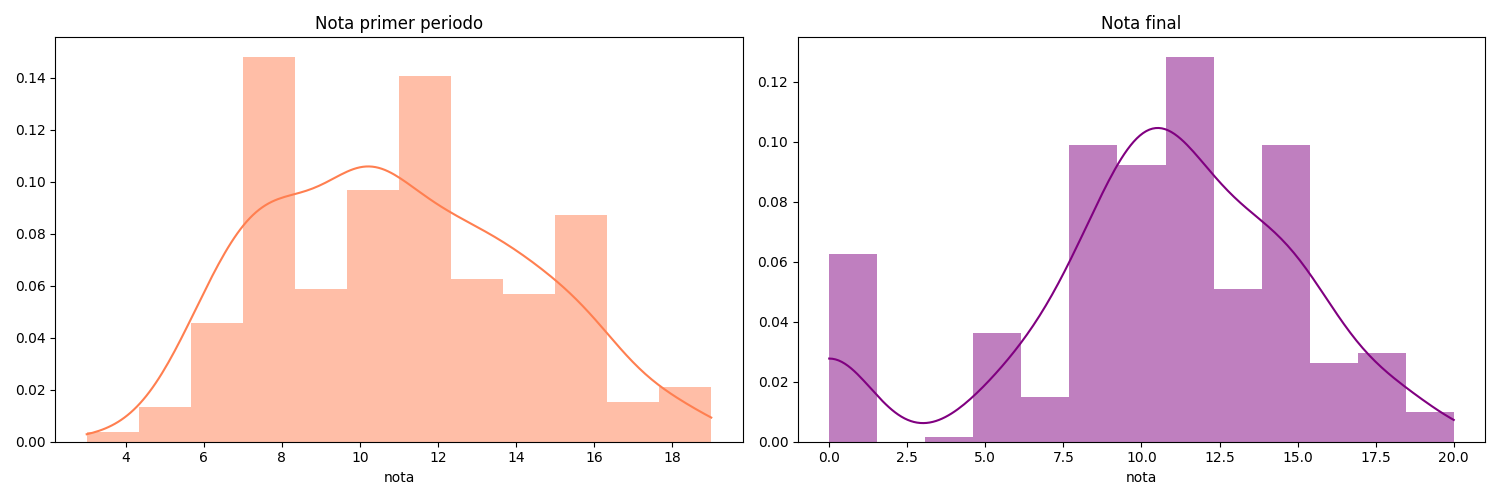
\includegraphics[width=1\textwidth]{./figures/dist-notas-alumnos.png}
    \caption{Gráficos de distribución de las notas de los alumnos}
    \label{fig:dist-notas}
\end{figure}

Si volvemos a realizar el test de Ómnibus d´Agostino obtenemos los siguientes resultados:
\begin{equation*}
    \begin{split}
        & K^2_{x} = 22.61 \Rightarrow \text{p-valor} = P(K^2 > 22.61) \approx 0\\ 
        & K^2_{y} = 32.05 \Rightarrow \text{p-valor} = P(K^2 > 32.05) \approx 0
    \end{split}
\end{equation*}

Aunque los estadísticos observados son más pequeños (denotando que las muestras son más anteriores que cuando veíamos las faltas en clase), los p-valores siguen siendo muy cercanos al cero.

\pagebreak

Sin embargo, como los datos son medianamente simétricos y además disponemos de una muestra suficientemente grande, utilizaremos un contraste paramétrico de diferencia de medias.
\begin{equation*}
    \begin{split}
        & \gamma_{1}(x) = \frac{\sum_{i=1}^{n}(x_i - \bar{x})^3}{n \cdot s^3} = 0.24\\
        & \gamma_{1}(y) = \frac{\sum_{i=1}^{n}(y_i - \bar{y})^3}{n \cdot s^3} = -0.73
    \end{split} 
\end{equation*}

Como estamos trabajando con muestras dependientes (medimos la nota del alumno en distintos momentos y además la nota final depende de la nota del primer y segundo periodo), utilizaremos un t-test de muestras pareadas.
\begin{itemize}
    \item \textbf{Hipótesis nula ($H_0$)}: $\mu_x - \mu_y = \mu_D = 0$ (no existe diferencias significativas entre la nota media del primer periodo y la nota media final)
    \item \textbf{Hipótesis alternativa ($H_a$)}: $\mu_x - \mu_y = \mu_D > 0$ (la nota media final mejora significativamente respecto a la nota media del primer periodo)
\end{itemize}

Al realizar el test obtenemos los siguientes resultados:
\begin{equation*}
    t_{obs} = 3.55 \Rightarrow \text{p-valor} = P(t_{394} > 3.55) = 0.0002
\end{equation*}

Por lo tanto, viendo que el p-valor es pequeño, concluimos que los datos muestran evidencias suficientes como para rechazar que la diferencia entre la media del primer periodo y la media final no es significativa. Aceptaremos la hipótesis alternativa de que la media final aumenta respecto a la del primer periodo.
